\chapter{Proposed Framework}
In this study we concentrate on automatic ensemble control of a special kind of devices: Thermostatically Controlled Loads (TCLs). We will use one-sided centralised incentive-based architecture with restrictions on the overall involvement of participating loads. 
\section{Thermostatically Controlled Loads}

\begin{definition}
    Thermostatically Controlled Loads (TCLs) is a type of loads who cycles through multiple stages according to the temperature of its subject of control.
\end{definition}
 This group includes water heaters, refrigerators, air conditioning systems, warm floors and many others. According to \cite{EIA2009}, a bit less than 50\% of energy in residential energy markets of USA is consumed by TCLs (see fig. \ref{fig:energy_consumption_in_usa}).

\begin{figure}
    \centering
    \label{fig:energy_consumption_in_usa}
    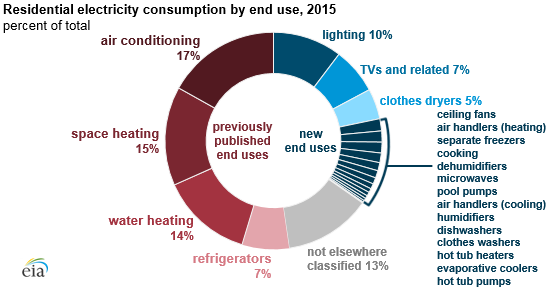
\includegraphics[width=0.9\textwidth]{figures/energy_consumption_in_usa}
    \caption{Residential energy consumption structure in United States, 2015}
\end{figure}

TCLs appear to be excellent candidates for participating in DR programs for at least four reasons:

\begin{enumerate}
    \item Insensitivity to short-term offs. As they naturally store energy in water tanks, short-term power outages almost do not affect consumers comfort.
    \item Descriptability by Markov Decision Processes. As was shown in \cite{Taylor2014, Chertkov2017}, such devices are naturally fit to Markov models due to the nature of physical process underlying their work.
    \item Availability in the majority of residential and commercial premises. 
    \item A big share of consumed energy (see \ref{fig:energy_consumption_in_usa}).
\end{enumerate}


\section{Markov Chain Modelling of Loads}

A common approach of dealing with uncertainty in Demand-Response is to model loads as Markov Chains (MCs). The viability of such models by many researchers. Firstly, a detailed survey on modelling of TCLs with MCs was conducted by \cite{Koch2011}, where a significant precision of such models was demonstrated in experiment. Secondly, in \cite{Trovato2015} an ensemble of refrigerators was modelled by MCs. And, finally, \cite{Wu2016} was introduced such models for Plug-in Electric Vehicles. This approach is widely used in DR programs when the aggregator lacks of communication infrastructure, especially in case of ensemble control approach \cite{Chertkov2017}. 

To provide some intuition let us give a simple example of such modelling. Consider an ideal air heater, which has three working modes: no heating ($Q_0$), moderate heating ($Q_1$) and maximum heating ($Q_2$) with an energy consumption vector $\widetilde{q} = [q_1, q_2, q_3] \in R^3$ for these modes respectively. Suppose that Air Heater moves from one mode to another according to some fixed transition matrix $P \in \R^{3 \times 3}$ of an ergodic Markov chain. (see fig\todo{add P fig and ref}). It is easy to see that the average heat stream from this heater will be $q^Tu$, where $u_P$ is a unit eigenvector of the matrix $P$. Within a short period when the outdoor temperature is fixed, due to the heat balance equations, it leads to some fixed indoor temperature $t$. Hence, each behaviour model $P$ defines average energy consumption and mean indoor temperature for each room. In the figure \ref{fig:matrices_example} one may see two different control matrices $P_1$ and $P_2$ representing two different behaviour models. 

\begin{figure}
    \centering
    \tikz[scale=3]{
        \begin{scope}[nodes={draw, ultra thick}]
            \node (agent) [rounded rectangle] {Agent};
            \node (environment) [right = of agent, rounded rectangle] {Environment};
        \end{scope}
        \path[->]
            (agent) edge [bend left] node [above] {$a_t$} (environment)
            (environment) edge [bend left] node [below] {$r_t, \, x_{t+1}, Q_{t+1}$} (agent); 
    }
    \label{fig:matrices_example}
\end{figure} 

\section{Notation and Problem Setup} We consider the system of $n$ thermostatically controlled loads, indexed by $i = 1, 2, \dots, n$. We suppose that there is an aggregator $A$ which send matrices ${\bar P}(t)$, $t=1, \dots, T$.

We refer $P_i(t) \in \mathbb{R}^{N\times N}$ as a transition matrix of load $i$, $i = 1, \dots, n$, and $N$ is a number of possible states of any load (all loads have the same number of states). Each load has its own behaviour defined as a function $P_i(t)$. All these behaviours are independent. We also suppose that any ${\bar P}(t)$ and $P_{i}(t)$  $\in {\cal P} = \{P^{(1)}, P^{(2)}, \dots, P^{(m)}\}$. Each load is allowed to accept or reject a transition matrix ${\bar P}(t)$ according to the following rule: 


\[
    {\bar P_i}(t) = 
    \begin{cases}
    {\bar P}(t), & \text{ if } \Omega(\bP(t),P_{i}(t), t) = 1\\
    P_i(t), & \text{otherwise},
    \end{cases}
\]

where $\Omega(P_1, P_2, t)$ is some decision rule which meets all legal and customer requirements. For the sake of simplicity we may assume this rule is known (i.e. a part of the contract), however, it is not required: we may learn it on-the-fly. Also, as we have only $m$ different matrices, $\Omega$ is a time-dependent matrix where $\Omega_{ij}(t) = 1$ if having own matrix $P_k(t) = P^{(i)}$ a load $k$ accepts proposed matrix $\bP^{(j)}$ at time t. 


%
We refer $\pi_i(t)$ as a unit vector corresponding to the state of load $i$, $1\le i \le n$, at time $t$, so that 
\[\pi(t) = \frac{1}{n}\sum_{i=1}^n \pi_i(t).\]
We also assume the the power consumption $q$ at each state is known, so that the total power consumption $s(t)$ is 
\[s(t) = n\cdot \pi(t)^\top q.\]
We refer ${\bar s}(t)$ as the power requested by the system operator at time $t$. 

We also assume the loss function of the system operator to be 
\[
\sum_{i=1}^T c(t) |{\bar s}(t) - s(t)|, 
\]
where $c(t) > 0$  is non-negative cost function. 



In this research we implement an incentive-based model of users motivation to participate in the curtailment program. In particular we consider the Emergency Demand-Response Program (EDRP) setting here, in which consumers get incentive payments for reducing their power consumption during reliability triggered events (see \cite{Aalami2010}). Consumers may choose not to curtail and therefore to forgo the payments, which are usually specified beforehand \cite{Vardakas2015}. Due to privacy protection reasons (\cite{Lisovich2010}) the aggregator is forbidden to observe exact loads accepting a curtailment request, but it is important to know the total amount of these loads for two reasons: 
    \begin{enumerate}
        \item As the aggregator's budget is strictly limited, it must estimate expenses for incentive payments. 
        \item Most of the DR incentive-based programs limit the total amount of curtailment hours to avoid user disturbance (typically 200 hours/year \cite{Aalami2010b})       
    \end{enumerate}
    
To sum up, the exact objective will be:

\begin{align}
    \label{optimization_setup}
    \min & \sum_{i=1}^T c(t) |{\bar s}(t) - s(t)| \\
    s.t. & \sum_{t=1}^T k(t) \leq K 
\end{align}

\section{Solution}
In the following section we treat \ref{optimization_setup} as a \textbf{linear contextual bandit with knapsack} problem \cite{Badanidiyuru2013}. Define the policy as some mapping from the context $f(t)$ to the matrix number $i \in \{0, 1, \dots, m\}$ (a.k.a. arm). The goal is to learn the policy $\nu$ which minimizes the regret:

\begin{equation}
    \begin{split}
    \min_{\nu}\, & {\cal R}^{\nu}_T = \min_{\nu} \sum_{t=1}^T(r^{\nu}(t) - r^*(t)) \\
     s.t. & \sum_{t=1}^T k(t) \leq K 
     \end{split}
\end{equation}
where the penalty is defined as
\[
    r^{\nu}(t) = c(t)|s^{\nu}(t) - {\bar s}(t)|
\]
and $k(t)$ is the number of loads who accepted the curtailment request at the time $t$, $K$ is the contract limit for user disturbance and $\nu$ is the policy being used. Hereafter we refer to $r^{\nu}(t)$ as $r(t)$.

In this form of bandits setup we face two major troubles: 
\begin{enumerate}
    \item General bandit with knapsack problem setup \cite{Badanidiyuru2013} consider penalties as a random independent variables over time and arms. Both assumptions here are false: our choices from the past strongly affects the current reward distributions.
    \item Variables $k(t)$ are unobservable, hence we can only ensure thresholds with some probability. 
\end{enumerate} 

To deal with these issues consider the the mechanics of how $s(t)$ depends on aggregator's actions. Suppose that by the time $t$ we have a (possibly unknown) state-distribution $\pi(t)$. It is easy to see that if each device chooses its own matrix, and we denote the number of devices which have chosen matrix $P_j$ as $n_j$, then the next-moment consumption with no control will be:

    \begin{equation}
    \label{eq:no_control_consumption}
        s(t|0) := \sum_{j=1}^{m}n_j(t)q^TP_j\pi(t) = \sum_{j=1}^{m}n_j(t)f_j(t|0)
    \end{equation}
    
    and if we pull $i^{th}$ arm, the consumption will be:

    \begin{equation}
        \label{eq:arm_consumption}
        s(t|i) := \sum_{j=1}^mn_j(t)q^T(\Omega_{ij}(t)P_i + (1-\Omega_{ij}(t))P_j)\pi(t) = \sum_{j=1}^{m}n_j(t)f_j(t|i)
    \end{equation}
    
    The model appears to be linear over unknown variables $n_j(t)$ and some vector $f(t|i) := \{f_j(t|i)\}_{j=1}^{m},\, i \in [0, 1, \dots m]$ which we know if we have $\pi(t)$ and $\Omega_{ij}(t)$. Therefore it is surprisingly convenient to consider $f(t|i)$ as a feature vector of an arm $i$ at the moment $t$. Note, that the features $f_j(i|t)$ have the natural interpretation as the amount of energy being consumed by an average device which has $\bP = P_j$ at the time $t$ if we pull the $i$-th arm. Moreover, we also have an estimator for budgeted variable: $k(t|i) = \sum_{i=1}^{m}\Omega_{ij}n_j$.


\paragraph{The Bandit} The above mentioned arm feature vectors (a.k.a. arm-contexts) $f(i|t)$ reveals a straightforward "linear contextual bandit with knapsack" setup:

\begin{align*}
    \label{eq:linear_bandits_with_context_setup}
    \min_{\nu:\, t \to \{0, 1\dots m\} }& \sum_{t=1}^T{\cal L}_t\left(n(t)^Tf(t|\nu(t))\right)\\
     s.t. \E&  \sum_{t=1}^T k(t|\nu(t)) \leq K \\
     & \sum_{j=1}^m n_j(t) = n\, \forall t\\
     & n_j(t) \geq 0\, \forall t
\end{align*}

where $n(t) = \{n_j(t)\}_{j=1}^m$ (do not miss it with $n$ -- the total amount of devices), and ${\cal L}_t(x)$ is a loss function. In this work two classical demand-response loss functions are considered. The first one is a trivial mapping:

\begin{equation}
    \label{eq:trivial_loss}
    {\cal L}_t(x) = x
\end{equation}
which gives the consumption minimization setup:

\begin{align}
    \label{eq:minimization_bandit_setup}
    \begin{split}    
    \min_{\nu:\, t \to \{0, 1\dots m\} }& \sum_{t=1}^Tn(t)^Tf(t|\nu(t)) = \min_{\nu} \sum_{t=1}^Ts^\nu(t)\\
     s.t. \E& \sum_{t=1}^T k(t|\nu(t)) \leq K \\
     & \sum_{j=1}^m n_j(t) = n\, \forall t\\
     & n_j(t) \geq 0\, \forall t
     \end{split}
\end{align}

and the second one is the absolute deviation from a given series $\bs(t)$:

\begin{equation}
    \label{eq:stabilization_loss}
    {\cal L}_t(x) = |x - \bs(t)|
\end{equation}
which gives the consumption stabilization setup:

\begin{align}    
    \begin{split}
    \label{eq:stabilization_bandit_setup}
    \min_{\nu:\, t \to \{0, 1\dots m\} }& \sum_{t=1}^T|n(t)^Tf(t|\nu(t)) - \bs(t)| = \min_{\nu } \sum_{t=1}^T|s^\nu(t) - \bs(t)|\\
     s.t. \E& \sum_{t=1}^T k(t|\nu(t)) \leq K \\
     & \sum_{j=1}^m n_j(t) = n\, \forall t \\
     & n_j(t) \geq 0\, \forall t
     \end{split}
\end{align}

It remains to notice that $n(t)$ is a periodic function over time with a period of 24 hours (at least within one season of a year), so we can consider \ref{eq:minimization_bandit_setup} and \ref{eq:stabilization_bandit_setup} as a set of 24 bandits: each one is learning to make a decision at the assigned hour. Note that these problems are in exact form for recently emerged budgeted bandit solvers (\cite{Badanidiyuru2013} and more (add later)), and all the requirements are met: the divergence between predicted and real consumption may appear only regarding to stochatical fluctuations due to the finiteness of the ensemble, hence we have independence of reward as a function of a context through arms and time (\textit{of course we need a proof here}). 


\paragraph{The Algorithm with known $\Omega_{ij}(t)$ and without a knapsack:} Consider a simpler setup when $K = \infty$ i.e. we have no knapsack constraints in our problem. Here $\tau$ is the number of steps which a device performs each hour. We also assume that we do not know neither an initial state distribution $\pi(0)$ nor $n_j(t)$. In this case \ref{algo:simple} is how a dummy algorithm may look like (we assume here a \ref{eq:stabilization_loss} loss function).

\begin{algorithm}
\caption{Non-budgeted TCL-control with oracle}
\label{algo:simple}
\begin{algorithmic}[1]
\REQUIRE{${\cal P},\, n,\, \tau, \Omega_{ij}(t)$}
\STATE{$n_i(0) := 1/n\, \forall i$}
\STATE{$\pi_0 := \frac{1}{n}\sum_{i=1}^mn_i(0)u_i$, where $u_i$ is a stationary distribution of the matrix $P_i$}
\STATE{$A(t) = \{\emptyset\} \, \forall t$ where A(t) is an array of all feature vectors through time which we got at the hour $t$. It will be used as a learning dataset for the $t$-th regressor.}
\STATE{$S(t) =  \{\emptyset\} \, \forall t$ where S(t) is an array of all s(t) through time which we got at the hour $t$. These are the targets for the $t$-th regressor.}
\FOR{$t := 1\dots T$}
    \STATE{Generate the arm contexts $\{f_j(t|i)\}_{j=1}^{m}$ for all $i \in \{0, 1\dots m\}$}:
    \STATE{$f_j(t|i) := \sum_{\xi = 1}^\tau q^T(\Omega_{ij}(t)P^{\xi}_i + (1-\Omega_{ij}(t))P^{\xi}_j)\pi(t)\quad i \in \{1\dots m\}$}
    \STATE{$f_j(t|0) := \sum_{\xi = 1}^\tau q^TP^{\tau}_j\pi(t)$}
    \IF{$\bs(t) == 0$}
        \STATE{Set $i := 0$ (no control) and send it to the ensemble}
    \ELSE
        \STATE{$i := \arg\max_{i\in \{1 \dots m\}} {\cal L}_t(s(t|i)) := \arg\max_{i\in \{1 \dots m\}}{\cal L}_t(n(t)^Tf(t|i))$}.
        \STATE{Send the chosen arm $i$ to the ensemble}
    \ENDIF
    \STATE{Wait and receive $s(t|i)$ -- the actual ensemble consumption}
        \STATE{$A(t)$.append($f(t|i)$)}
        \STATE{$S(t)$.append($s(t|i)$)}
        \STATE{Solve a constrained regression problem to learn real $n_j(t)$:}
        \STATE{$n(t) = \arg \min_{n \in R^n_+} \|A(t)n(t) - S(t)\|^2, \, s.t. \sum_{j=1}^m n_j(t) = n,\, n_j(t) \geq 0,\, \text{start from } n(t)$}
        \STATE{Calculate next $\pi$:}
        \STATE{$\pi(t+1) = \frac{1}{n}\sum_{j=1}^mn_j(t)(\Omega_{ij}(t)P^{\tau}_i + (1-\Omega_{ij}(t))P^{\tau}_j))\pi(t)$}
        \IF{$n_j(t+1)$ are undefined yet}
            \STATE{$n_j(t+1) = n_j(t)$}
        \ENDIF
\ENDFOR
\end{algorithmic}
    
\end{algorithm}


One may notice that in \ref{algo:simple} the greedy policy was used, and no exploration steps were proposed. In fact, the greedy policy here turns to be optimal: all the reward variances depend only on unknown vector $n(t)$ and when we learn it we decrease reward variances for all arms simultaneously. Hence, in contrast to the following case, no exploration-exploitation balance is required here. 

\paragraph{The Algorithm without a knapsack and without $\Omega_{ij}(t)$} Note that it is not crucial for the previous algorithm to know the oracle $\Omega_{ij}(t)$, as we may learn in the same way we learn $n(t)$. Formally, let $i$ be the arm the aggregator pulled at the moment $t$, then the consumption will be:

    \begin{equation}
        \begin{split}
            s(t|i) = & n(t)^Tf(t|i) = \sum_{j=1}^m n_j(t)\sum_{\xi = 1}^\tau q^T(\Omega_{ij}(t)P^{\xi}_i + (1-\Omega_{ij}(t))P^{\xi}_j)\pi(t) = \\
            & = \sum_{j=1}^m\Omega_{ij}(t) n_j \sum_{\xi = 1}^{\tau}q^T(P_i^\xi-P_j^\xi)\pi(t) + \underbrace{\sum_{j=1}^{m}n_j\sum_{\xi=1}^\tau q^TP_j^\xi\pi(t)}_{s(t|0)}
        \end{split}
    \end{equation}
    
    and we have a discrete regularized regression problem over the vector $\Omega_{i}(t) \in \{0, 1\}^m$ here:
    
    \begin{equation}
        \underbrace{s(t|i) - s(t|0)}_{target} = \sum_{j=1}^m\underbrace{\Omega_{ij}(t)}_{variables} \underbrace{n_j(t)\sum_{\xi=1}^\tau q^T(P_i^\xi - P_j^\xi)\pi(t)}_{features}
    \end{equation}
    
    
 If we also have observations from $i$-th arm at $t$-th hour from the past (i.e. this is not the first time we pull this arm at this hour), then we may solve the least-squared optimization problem over $\Omega_{ij}(t)|_{j=j} \in \{0, 1\}^m$ which might reduce the fluctuations of $\Omega$. 
 
 The algorithm \ref{algo:non_budgeted_without_oracle} for this case is the essentially the same: the new parts are marked with {\color{red} red}.
\begin{algorithm}
\caption{Non-budgeted TCL-control without oracle}
\label{algo:non_budgeted_without_oracle}
\begin{algorithmic}[1]
\REQUIRE{${\cal P},\, n,\, \tau,$ {\color{red} \st{$\Omega_{ij}(t)$}}}
\STATE{$n_i(0) := 1/n\, \forall i$}
\STATE{$\pi_0 := \frac{1}{n}\sum_{i=1}^mn_i(0)u_i$}
\STATE{$A(t) = \{\emptyset\} \, \forall t$}
\STATE{$S(t) =  \{\emptyset\} \, \forall t$}
\STATE{{\color{red}$\Omega_{ij}(0) = \{0,1\}^{m\times m}$ -- random matrix}}
\FOR{$t := 1\dots T$}
    \STATE{Generate arm contexts $\{f_j(t|i)\}_{j=1}^{m}$ for all $i \in \{0, 1\dots m\}$}:
    \STATE{$f_j(t|i) := \sum_{\xi = 1}^\tau q^T(\Omega_{ij}(t)P^{\xi}_i + (1-\Omega_{ij}(t))P^{\xi}_j)\pi(t)\quad i \in \{1\dots m\}$}
    \STATE{$f_j(t|0) := \sum_{\xi = 1}^\tau q^TP^{\tau}_j\pi(t)$}
    \IF{$\bs(t) == 0$}
        \STATE{Set $i := 0$ (no control) and send it to the ensemble}
        \STATE{Wait and receive $s(t|0)$ -- the actual ensemble consumption}
        \STATE{{\color{red} When we have no control signal, we learn $n_j(t)$}}
        \STATE{$A(t)$.append($f(t|0)$)}
        \STATE{$S(t)$.append($s(t|0)$)}
        \STATE{Solve a constrained regression problem to learn real $n_j(t)$:}
        \STATE{$n(t) = \arg \min_{n \in R^n_+} \|A(t)n(t) - S(t)\|^2, \, s.t. \sum_{j=1}^m n_j(t) = n,\, n_j(t) \geq 0,\, \text{start from } n(t)$}
        \STATE{Calculate next $\pi$:}
        \STATE{$\pi(t+1) = \sum_{j=1}^mn_j(t)P^{\tau}_j\pi(t)$}
    \ELSE
        \STATE{{\color{red} Calculate $s(t|i) = n(t)^Tf(t|i)$ for all $i \in \{0, 1, \dots m\}$}}
        \STATE{{\color{red} Calculate variance estimations $\Delta s(t|i)$}}
        \STATE{{\color{red} $i := \arg\min_{j \in \{0, 1, \dots m\}} {\cal L}_t(s(t|j) + B\sqrt{\Delta s(t|i)})$}}
        \STATE{Send the chosen arm $i$ to the ensemble}
        \STATE{Wait and receive $s(t|i)$ -- the actual ensemble consumption}
        \STATE{{\color{red} Learn the vector $\Omega_{i}(t)$ solving optimization problem:}}
        \STATE{{\color{red} $\Omega_i(t) := \arg \min_{\omega \in \{0, 1\}^m}\left(\underbrace{(s(t|i) - s(t|0))}_{s} - \sum_{j=1}^m\omega_j \underbrace{n_j(t)\sum_{\xi=1}^\tau q^T(P_i^\xi - P_j^\xi)\pi(t)}_{g_j}\right)^2 = $}}
        \STATE{{\color{red} $ = \arg \min_{\omega \in \{0, 1\}^m} \left(s - w^Tg \right)^2$}}
        \STATE{{\color{red} \textit{I suppose we need some kind of smooth  relaxation here}}}
        \STATE{Calculate next $\pi$:}
        \STATE{$\pi(t+1) = \frac{1}{n}\sum_{j=1}^mn_j(t)(\Omega_{ij}(t)P^{\tau}_i + (1-\Omega_{ij}(t))P^{\tau}_j))\pi(t)$}
    \ENDIF
    
        \IF{$n(t+1)$ is undefined yet}
            \STATE{$n(t+1) = n(t)$}
        \ENDIF
        \IF{$\Omega_{ij}(t+1)$ is undefined yet}
            \STATE{$\Omega_{ij}(t+1) = \Omega_{ij}(t)$}
        \ENDIF
\ENDFOR
\end{algorithmic}
\end{algorithm}


\paragraph{The Algorithm with a knapsack and without $\Omega_{ij}(t)$} This one is our final result. Note that we just need to apply not a regular UCB1 bandit inside the abovementioned algorithm, but the "bandit-with-knapsack" solver from \cite{Badanidiyuru2013} or something similar. 